\documentclass[8pt]{beamer}
\usetheme{Madrid}
\usefonttheme{serif}

\usepackage{fontspec}
% надёжный шрифт с кириллицей (работает в Overleaf)
\setmainfont{Libertinus Serif}[Ligatures=TeX]
\setsansfont{Libertinus Sans}[Ligatures=TeX]
\newfontfamily\cyrillicfont{Libertinus Serif}
\newfontfamily\cyrillicfontsf{Libertinus Sans}
\usepackage{polyglossia}
\setmainlanguage{russian}
\setotherlanguage{english}

\usepackage{amsmath}
\usepackage{amsfonts}
\usepackage{amssymb}
\usepackage{graphicx}
\usepackage{microtype}

\usepackage{tabularx}
\usepackage{booktabs}

\usepackage{xcolor}
\usepackage{pifont}
\usepackage{tikz}
\newcommand{\plus}{\tikz[baseline=(X.base)] \node[fill=green!65!black, rounded corners=2pt, inner sep=2pt] (X) {\color{white}\ding{51}};}
\newcommand{\minus}{\tikz[baseline=(X.base)] \node[fill=red!70!black,   rounded corners=2pt, inner sep=2pt] (X) {\color{white}\ding{55}};}

\DeclareMathOperator{\sen}{sen}
% \DeclareMathOperator{\tg}{tg}

\setbeamertemplate{caption}[numbered]

% --- Информация о презентации ---
\author[Автор]{Чиняев Владимир Николаевич}
\title{Основы полуаналитических методов \\ прогноза баллистического движения}
\newcommand{\coursename}{Введение в маневрирование КА}
\setbeamertemplate{navigation symbols}{} 
\institute[]{Московский физико технический институт} 
\date{9 декабря 2025 г.} 

\bibliographystyle{apalike}

% --- Кастомная нижняя синяя полоска: курс слева, номер слайда справа ---
\setbeamertemplate{footline}{
  \leavevmode%
  \begin{beamercolorbox}[wd=\paperwidth,ht=2ex,dp=1ex]{palette primary}
    \hspace{0.4cm}\usebeamerfont{footline}\coursename\hfill\usebeamerfont{footline}\insertframenumber\hspace{0.4cm}
  \end{beamercolorbox}%
}

% Чтобы убрать лишние отступы в footer-шрифте (опционально)
\setbeamerfont{footline}{size=\small}

\usepackage{ragged2e}
\apptocmd{\frame}{}{\justifying}{}

\begin{document}

\begin{frame}
\titlepage
\end{frame}

\begin{frame}{Возмущения орбитальных элементов}
\begin{center}
    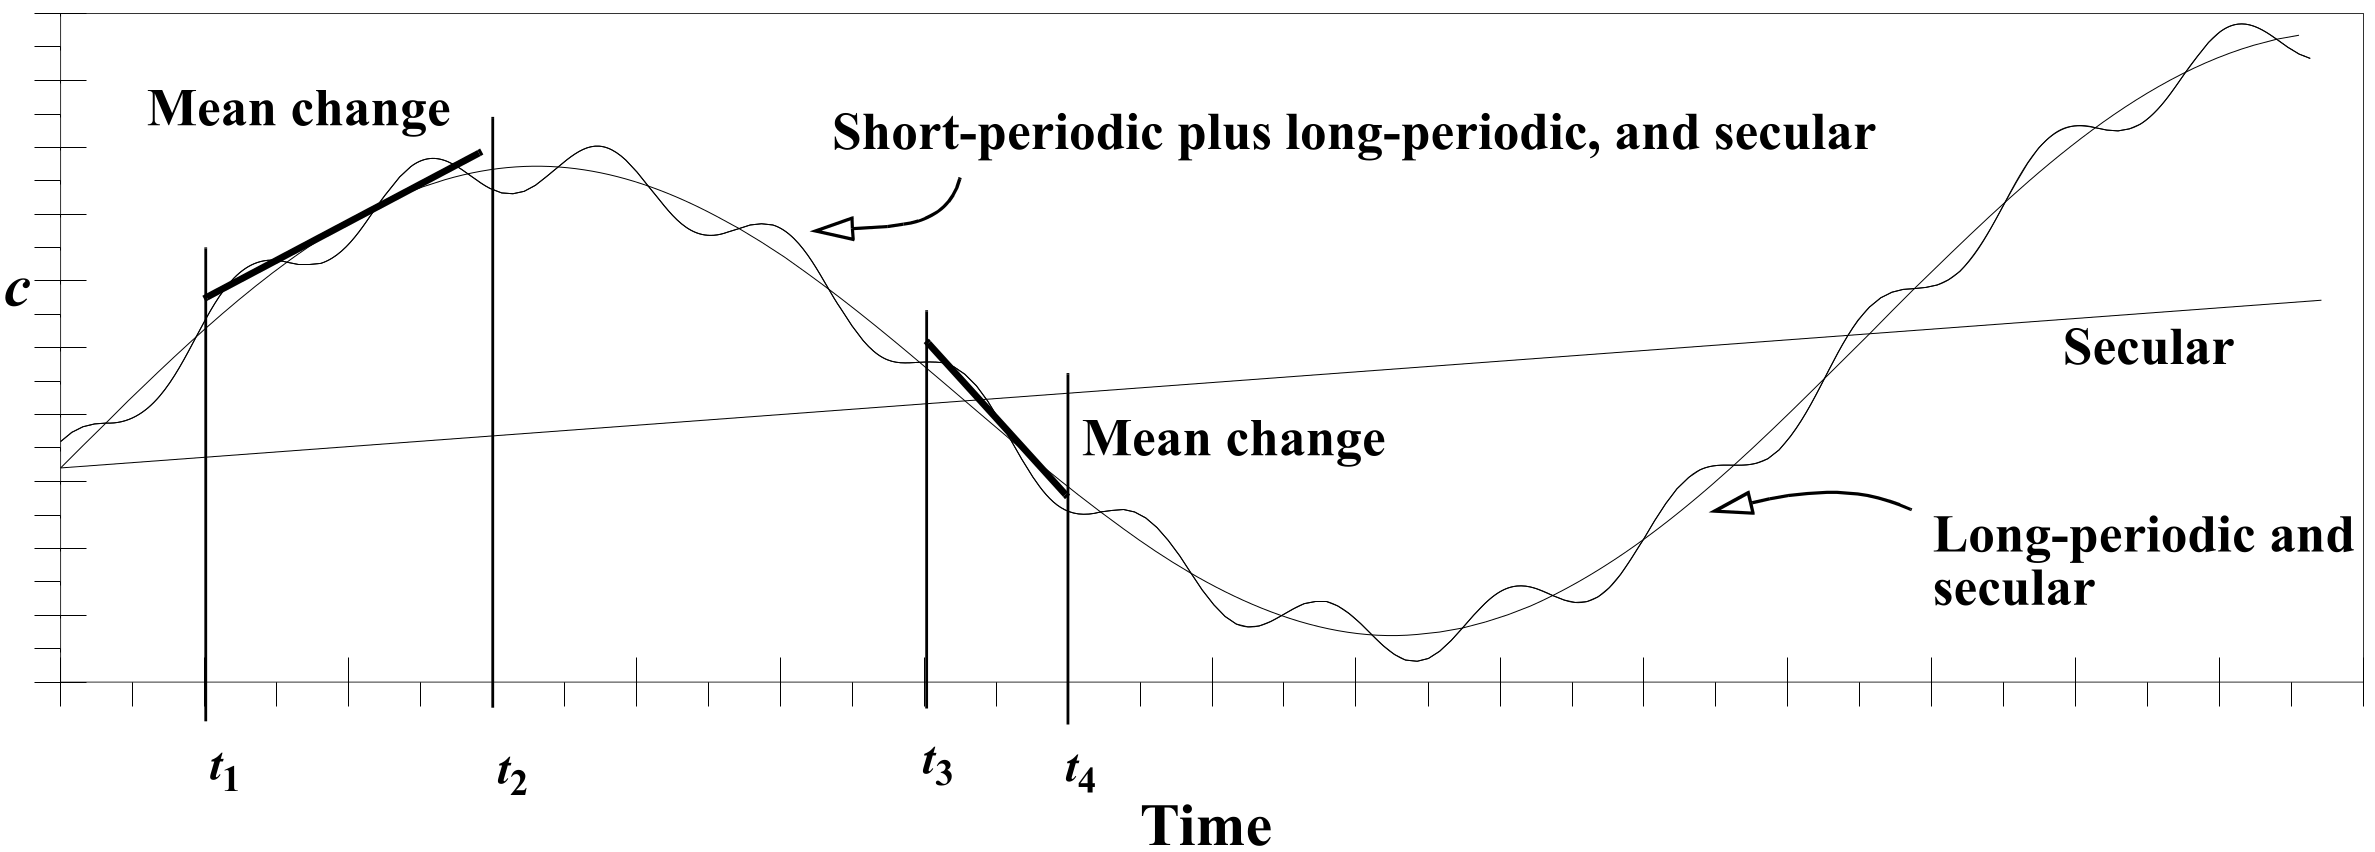
\includegraphics[height=0.45\textheight,keepaspectratio]{images/11/pert_types.png}
\end{center}
\textbf{Вековые возмущения} - это изменения орбитальных элементов, которые монотонно возрастают со временем. Именно из-за вековых возмущений ошибка в положении КА при аналитическом прогнозе растёт неограниченно. \\
\textbf{Долгопериодические возмущения} - это периодические изменения орбитальных элементов, период которых существенно больше орбитального периода спутника (обычно на $1-2$ порядка). Долгопериодические эффекты часто проявляются в движении линии узлов и перицентра и могут продолжаться от нескольких недель до месяца и более. \\
\textbf{Короткопериодические возмущения} - это периодические изменения орбитальных элементов, период которых сравним с орбитальным периодом спутника или меньше. Короткопериодические вариации возникают, когда во входящем в возмущающее воздействие выражении присутствует «быстрая» переменная (например, истинная аномалия). Именно короткопериодические возмущения задают минимальный шаг интегрирования в численных расчётах.
\end{frame}

\begin{frame}{Возмущения орбитальных элементов}
\begin{center}
    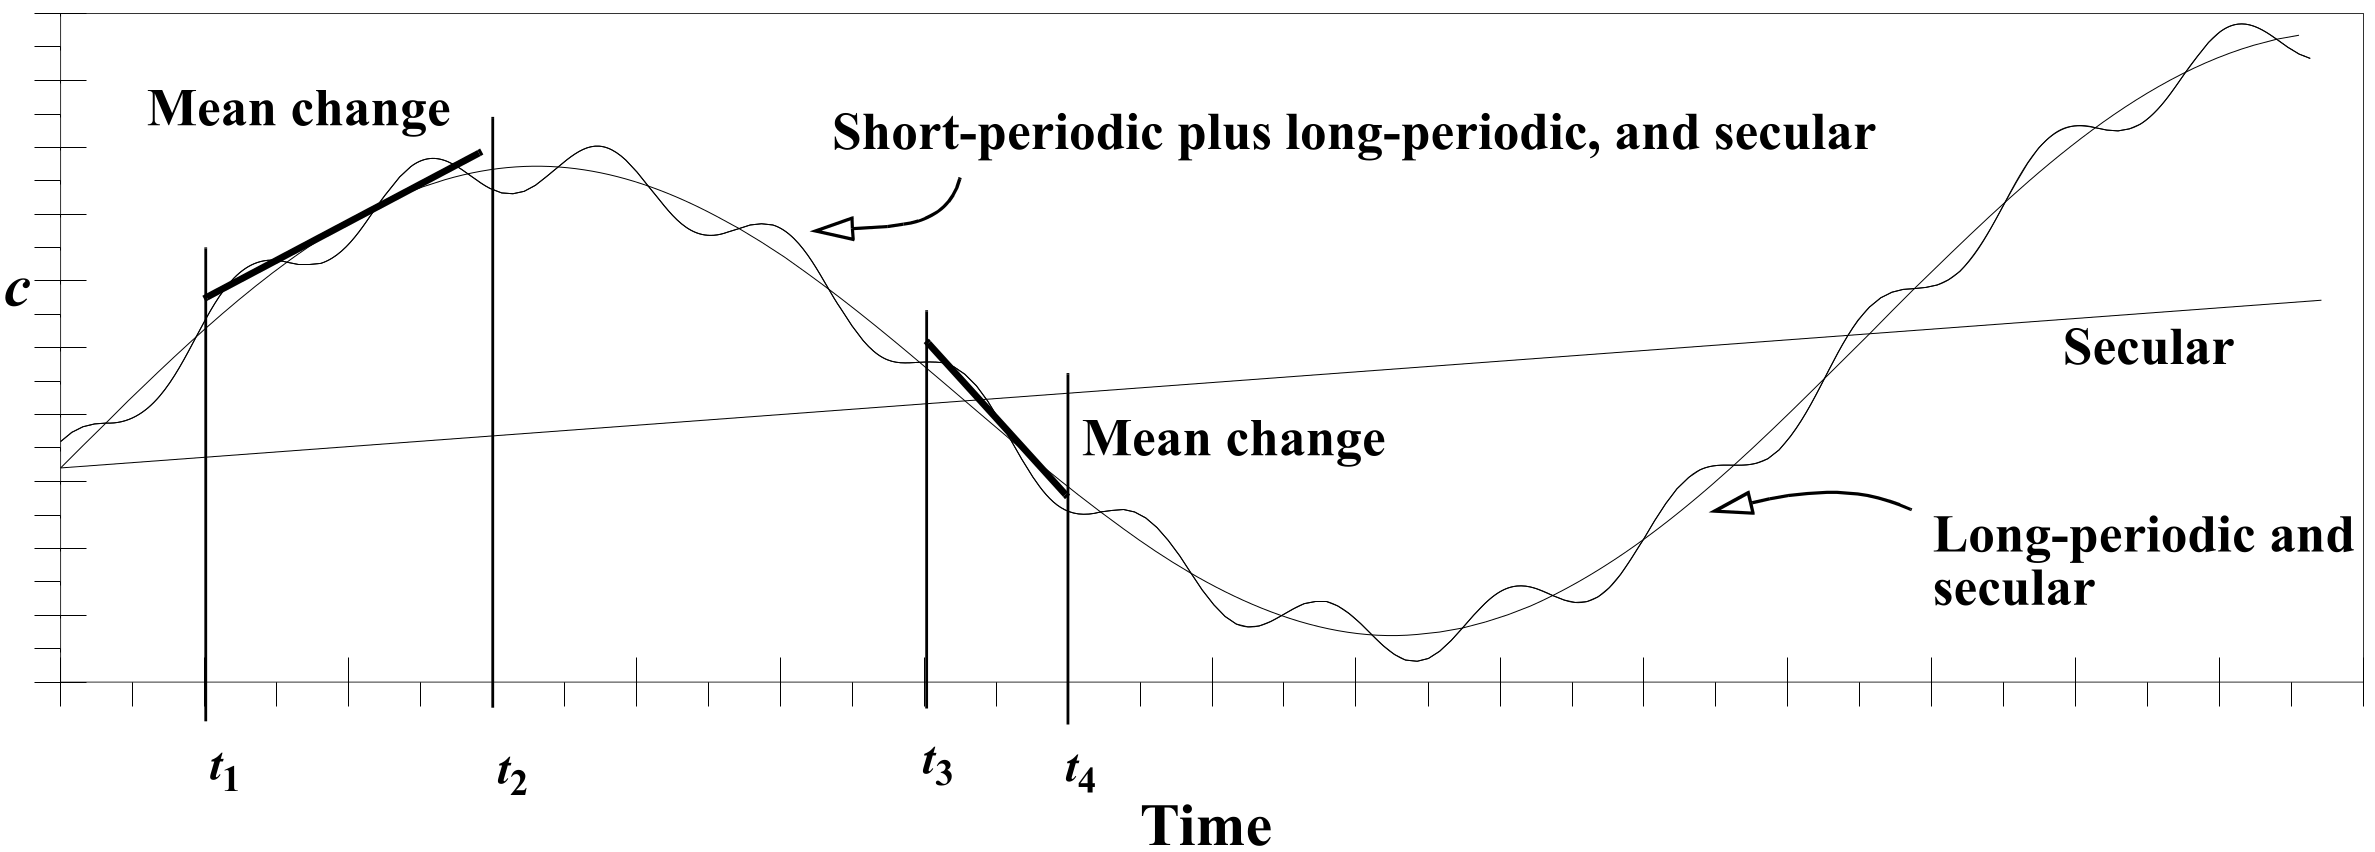
\includegraphics[height=0.45\textheight,keepaspectratio]{images/11/pert_types.png}
\end{center}
Нам также нужно различать некоторые орбитальные элементы как \textbf{быстрые} или \textbf{медленные} переменные в зависимости от их относительной скорости изменения. 
\begin{itemize}
    \item \textbf{Быстрые переменные} \\
    Заметно изменяются за один виток даже при отсутствии возмущений. Например:
    \begin{itemize}
        \item Средняя аномалия $M$, истинная аномалия $\nu$, эксцентрическая аномалия $E$, каждая из которых изменяется на $360^\circ$;
        \item Декартовы координаты.
    \end{itemize}

    \item \textbf{Медленные переменные} \\
    Изменяются очень мало за один орбитальный виток. Эти изменения вызываются возмущениями. Без возмущений все медленные элементы оставались бы постоянными. Быстрые переменные при этом продолжали бы изменяться. Например: большая полуось $a$, эксцентриситет $e$, наклонение $i$, долгота восходящего узла $\Omega$, аргумент перицентра $\omega$.
\end{itemize}
\end{frame}

\begin{frame}{Возмущения орбитальных элементов}
\begin{center}
    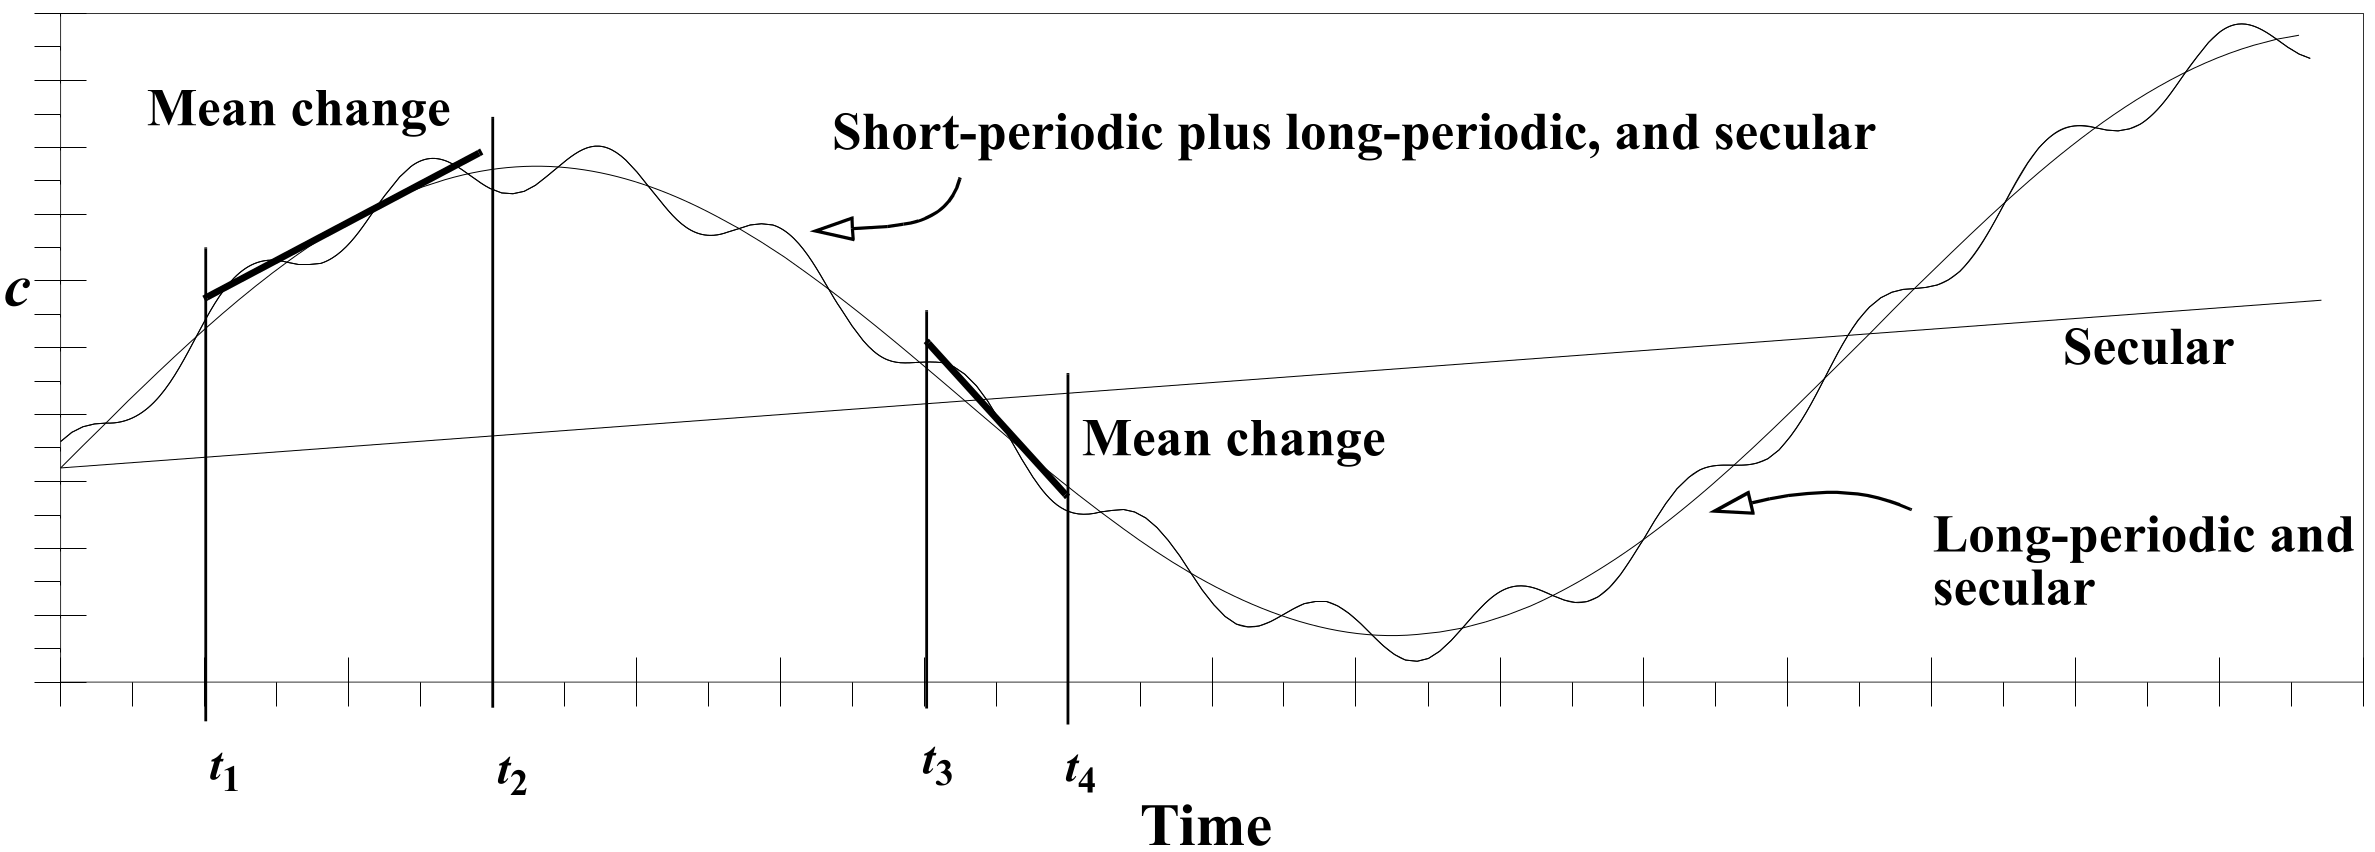
\includegraphics[height=0.45\textheight,keepaspectratio]{images/11/pert_types.png}
\end{center}
Мы можем описывать возмущённое движение спутника с помощью упорядоченной последовательности векторов положения и скорости. Соответственно, в каждый момент времени мы можем по этим векторам восстановить орбитальные элементы, используя методы задачи двух тел. Соответствующие векторы положения и скорости определяют в этот момент \textbf{оскулирующие элементы}. \\

Мы определяем \textbf{оскулирующую эллиптическую орбиту} как орбиту задачи двух тел, по которой спутник стал бы двигаться, если бы возмущающие силы в данный момент внезапно исчезли. \textbf{Оскулирующие элементы} — это истинные, зависящие от времени орбитальные элементы; они включают в себя все кратко- и долгопериодические, а также вековые возмущения. \\

В отличие от них, \textbf{средние элементы} получаются путём усреднения по некоторому выбранному интервалу времени, так что они меняются относительно плавно. Средние элементы зависят от некоторого, в общем случае неуточнённого, интервала усреднения по времени или углу.
\end{frame}

\begin{frame}{Методы прогноза баллистического движения}
\begin{columns}
    \begin{column}{0.50\textwidth}
        \begin{center}
            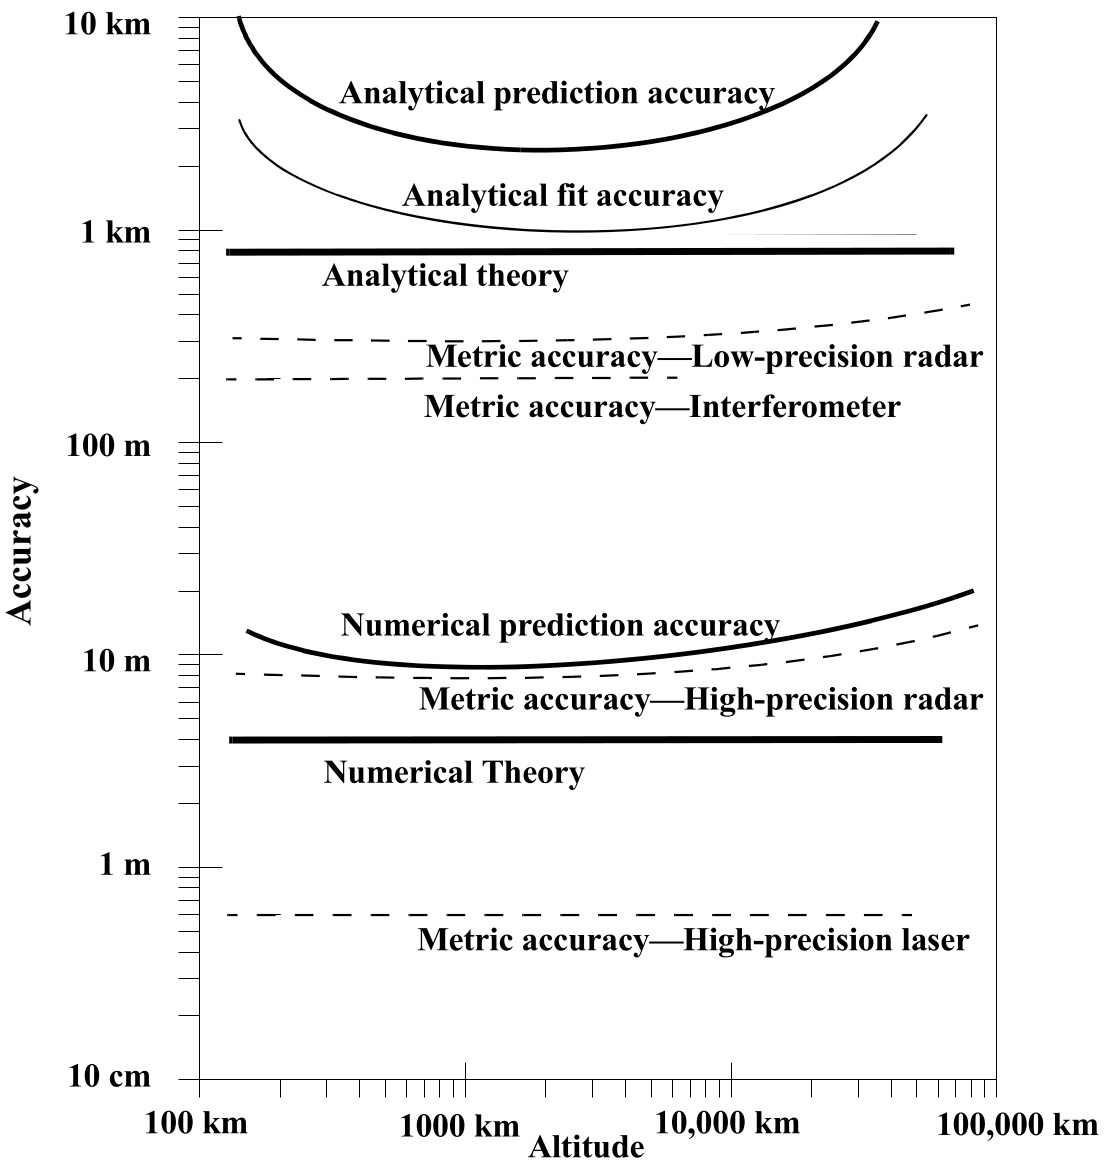
\includegraphics[height=0.75\textheight,keepaspectratio]{images/11/accuracy.png}
        \end{center}
    \end{column}

    \begin{column}{0.50\textwidth}
        \begin{center}
            \textbf{Аналитические методы}
        \end{center}
        \begin{itemize}
            \justifying
            \item Решение в виде рядов по малым параметрам возмущений; уравнения движения
            заменяются \emph{аналитическим приближением}.
            \item Точность ограничена порядком разложения и усечением рядов: вековые члены дают рост ошибки с временем.
            \item \plus\ Очень высокая скорость вычислений;
            \item \plus\ Единая формула для всего множества начальных условий; 
            \item \plus\ Хорошее качественное понимание влияния возмущений.
            \item \minus\ Сложная разработка; 
            \item \minus\ Трудно учитывать большой набор сил;
            \item \minus\ Область применимости по времени и по параметрам орбиты ограничена.
        \end{itemize}
    \end{column}
\end{columns}
\end{frame}

\begin{frame}{Методы прогноза баллистического движения}
\begin{columns}
    \begin{column}{0.50\textwidth}
        \begin{center}
            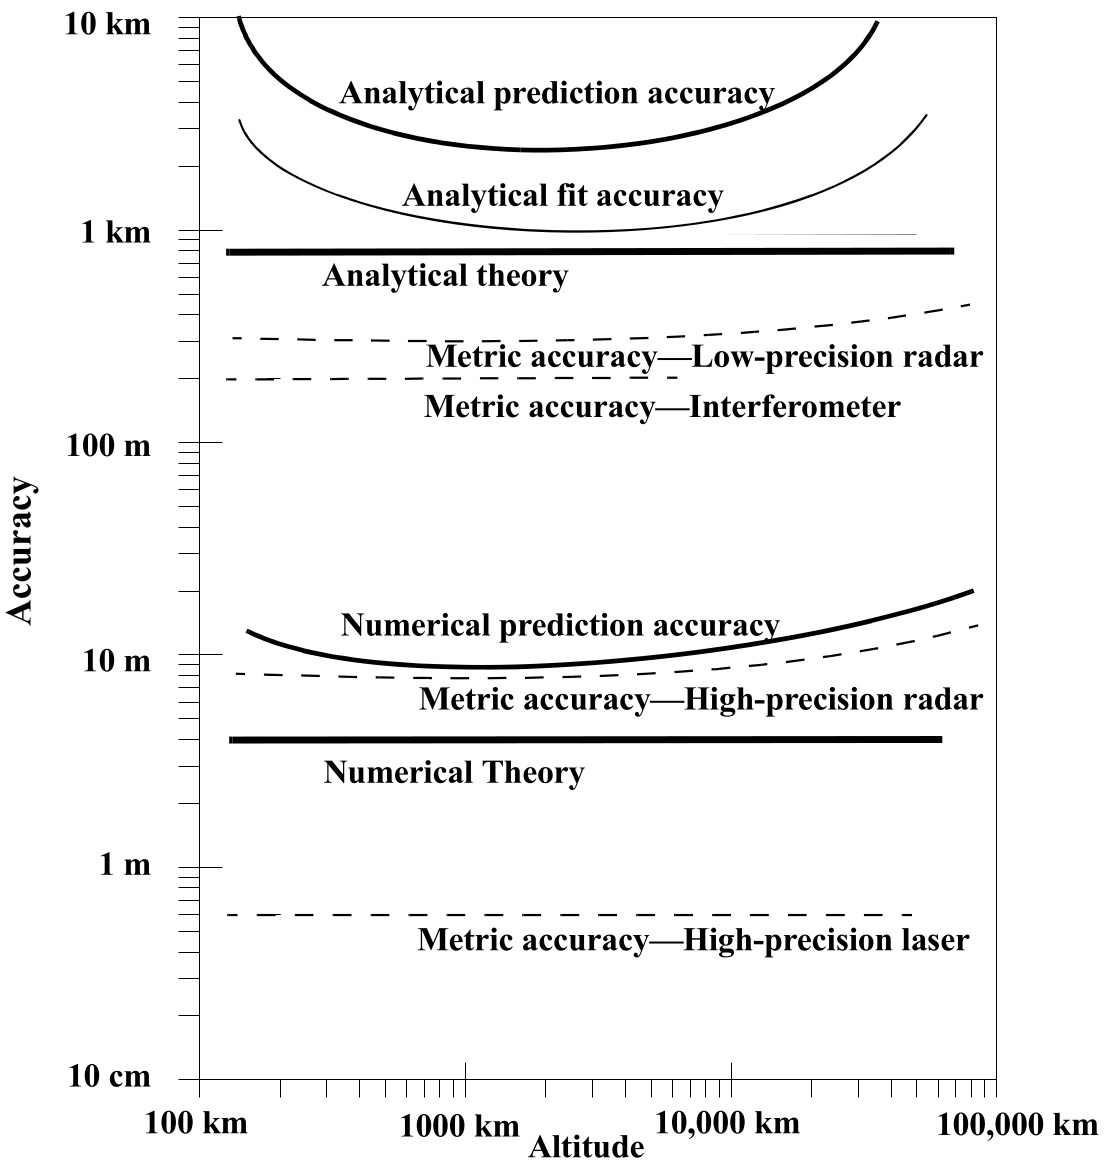
\includegraphics[height=0.75\textheight,keepaspectratio]{images/11/accuracy.png}
        \end{center}
    \end{column}

    \begin{column}{0.50\textwidth}
        \begin{center}
            \textbf{Численные методы}
        \end{center}
        \begin{itemize}
            \justifying
            \item Прямое интегрирование вектора состояния с полным набором моделей сил.
            \item При достаточно маленьком шаге и хорошем интеграторе обеспечивается очень высокая точность, но ошибка накапливается из-за шага интегрирования и округления.
            \item \plus\ Гибкость по силам;
            \item \plus\ Получение эталонной траектории; 
            \item \plus\ Легко повысить точность за счёт шага и порядка метода.
            \item \minus\ Высокая вычислительная стоимость при длительном интервале прогноза;
            \item \minus\ Слабая наглядность;
            \item \minus\ Шаг ограничен короткопериодическими эффектами.
        \end{itemize}
    \end{column}
\end{columns}
\end{frame}

\begin{frame}{Методы прогноза баллистического движения}
\begin{columns}
    \begin{column}{0.50\textwidth}
        \begin{center}
            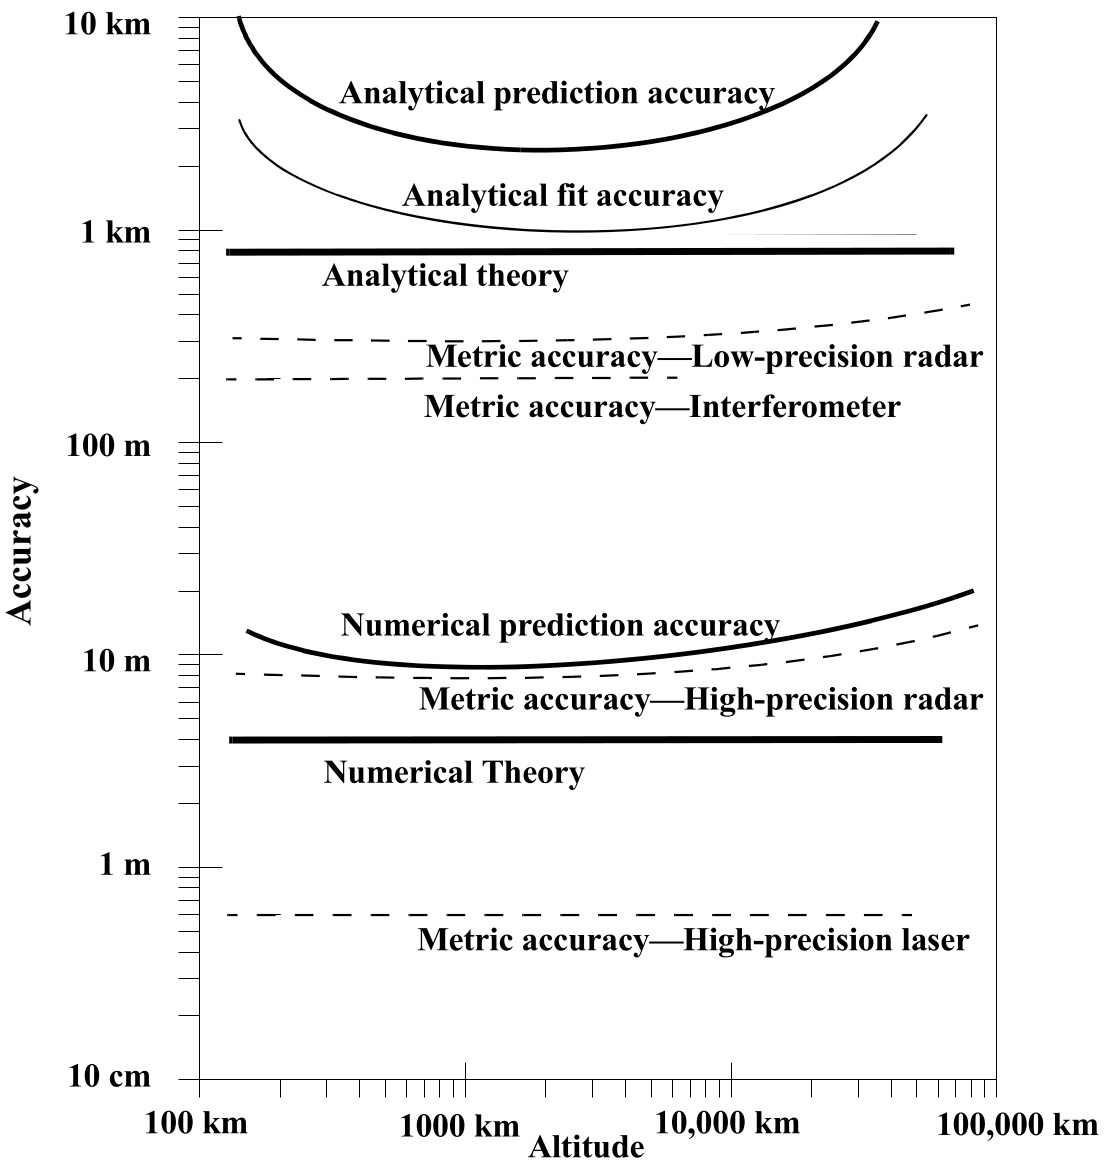
\includegraphics[height=0.75\textheight,keepaspectratio]{images/11/accuracy.png}
        \end{center}
    \end{column}

    \begin{column}{0.50\textwidth}
        \begin{center}
            \textbf{Полуаналитические методы}
        \end{center}
        \begin{itemize}
            \justifying
            \item Усреднение по быстрым переменным, аналитический учёт короткопериодических членов; численное интегрирование только медленных (средних) элементов.
            \item Достигают точности, близкой к численным методам, при существенно меньших затратах, но качество зависит от выбранной теории и числа учитываемых сил.
            \item \plus\ Хороший компромисс «точность/стоимость»; 
            \item \plus\ Удобны для долгосрочного прогноза и массовых расчётов.
            \item \minus\ Сложная реализация и отладка; 
            \item \minus\ Есть как аналитическая, так численная составляющая ошибки; 
            \item \minus\ Сильно зависят от качества документации и реализации.
        \end{itemize}
    \end{column}
\end{columns}
\end{frame}

\begin{frame}{Метод возмущений}
\textbf{Метод возмущений} (The Method of Perturbations) - набор математических приёмов, позволяющих получить аналитическую аппроксимацию решения уравнений движения при наличии возмущающих сил. \\
\smallskip
Концепция метода возмущений заключается в том, что одна или несколько возмущающих сил вызывают малые отклонения от известного решения для невозмущённой задачи. Эти малые возмущающие силы могут быть связаны с малыми параметрами, определяющими величину возмущающих сил:
\begin{equation*}
    \frac{dc_i}{dt} = \epsilon_1 f_i + \epsilon_2 g_i, \quad \epsilon_1 \ll 1, \quad \epsilon_2 \ll 1,
\end{equation*}
где $c_i$ - элементы орбиты; $f_i$, $g_i$ описывают действие возмущающих сил; $\epsilon_1$, $\epsilon_2$ - малые параметры, характеризующие их величину.
\end{frame}

\begin{frame}{Метод возмущений}
Приближение к реальному решению может быть получено как 
\begin{equation*}
\begin{aligned}
    c &= c_0 + \epsilon_1 \alpha_1(t) + \frac{\epsilon_1^{2}}{2!} \alpha_2(t) + \dots \\
      &\quad + \epsilon_2 \beta_1(t) + \frac{\epsilon_2^{2}}{2!} \beta_2(t) + \dots \\
      &\quad + \frac{\epsilon_1 \epsilon_2}{2!} \gamma_2(t) + \dots
\end{aligned}
\end{equation*}
Здесь $c_0$ - невозмущённое решение (орбита задачи двух тел), $\alpha_k$, $\beta_k$, $\gamma_k$ - поправки, зависящие от времени. \\
\smallskip
\textbf{Порядок теории} — это максимальная степень малого параметра, до которой сохраняют члены в разложении.
\begin{itemize}
    \item Теория первого порядка — учёт только членов $\sim \epsilon$;
    \item Теория второго порядка — учёт членов $\sim \epsilon^2$ и т.д.
\end{itemize}
В основе — обычное разложение в ряд Тейлора, это ядро всех решений методом возмущений. \\
\smallskip
\textbf{Примеры малых коэффициентов:}
\begin{itemize}
    \item Коэффициенты разложения гравитационного потенциала Земли: $\text{J}_2$, $\text{J}_3$, $C_{lm}$, $S_{lm}$;
    \item Отношение больших полуосей спутника и третьего тела ($\frac{a}{a_3}$) для возмущений от третьих тел;
    \item Безразмерные параметры лобового сопротивления, тяги, давления света и т.п.
\end{itemize}
Для достаточно малых $\epsilon$ такие ряды хорошо сходятся на конечном интервале времени.
\end{frame}

\begin{frame}{Метод вариации параметра}
\begin{columns}
    \begin{column}{0.50\textwidth}
        \justifying
        \textbf{Метод вариации параметра} (variation of parameters, VOP) — это такая форма записи уравнений движения, которая хорошо подходит для возмущённых динамических систем. Идея основана на предположении, что мы можем использовать решение для невозмущённой системы, чтобы представить решение возмущённой системы, если обобщим постоянные в этом решении до параметров, зависящих от времени. \\
        \begin{center}
            \textbf{Невозмущённая задача двух тел}
        \end{center}
        \begin{equation*}
            \ddot{\mathbf{r}} = -\frac{\mu}{r^3} \mathbf{r}.
        \end{equation*}
        Существует аналитическое решение в параметрической форме:
        \begin{equation*}
            \mathbf{x}(t) =
            \begin{bmatrix}
              \mathbf{r}(t) \\
              \mathbf{v}(t)
            \end{bmatrix}
            =
            \hat{\mathbf{x}}(\mathbf{c}, t),
        \end{equation*}
        где $\mathbf{c} \in \mathbb{R}^6$ — набор констант невозмущённого движения (орбитальные элементы или иной полный набор интегралов).
    \end{column}

    \begin{column}{0.50\textwidth}
    \begin{center}
        \textbf{Возмущённая задача}
    \end{center}
    \begin{equation*}
        \ddot{\mathbf{r}} = -\frac{\mu}{r^3}\,\mathbf{r} + \mathbf{a}_{\text{pert}}(\mathbf{r}, \mathbf{v}, t).
    \end{equation*}
    Идея метода вариации постоянных (VOP):
    \begin{equation*}
        \mathbf{c} = \mathbf{c}(t), \qquad
        \mathbf{x}(t) = \hat{\mathbf{x}}(\mathbf{c}(t), t).
    \end{equation*}

    \begin{center}
        \textbf{Связь с уравнениями движения}
    \end{center}
    \begin{equation*}
        \dot{\mathbf{x}} = \frac{\partial \hat{\mathbf{x}}}{\partial t} + \sum_{i=1}^{6} \frac{\partial \hat{\mathbf{x}}}{\partial c_i}\,\dot c_i,
    \end{equation*}
    \begin{equation*}
        \frac{d\mathbf{c}}{dt} 
        = \mathbf{f}(\mathbf{c}, t) 
        = \mathbf{G}(\mathbf{c}, t)\,\mathbf{a}_{\text{pert}}(\mathbf{r}, \mathbf{v}, t),
    \end{equation*}
    где $\mathbf{G}$ определяется выбором параметров $\mathbf{c}$ и условием оскуляции.
    В невозмущённом случае $\mathbf{a}_{\text{pert}} = \mathbf{0}$, и $\dot{\mathbf{c}} = \mathbf{0}$.
    \end{column}
\end{columns}
\end{frame}

\begin{frame}{Аналитические методы}
\textbf{Общая идея}
\begin{itemize}
\justifying
  \item Исходная задача: уравнения движения сведены к уравнениям для орбитальных
        элементов (метод вариации постоянных).
  \item В аналитических теориях движение представляют в виде рядов по малым
        параметрам возмущений и по гармоникам:
        \[
          c(t) = c_0
                 + \dot c_{\text{век}}\,t
                 + \Delta c_{\text{SP}}(t)
                 + \Delta c_{\text{LP}}(t),
        \]
        где SP/LP — коротко- и долгопериодические члены. 
  \item Короткопериодические члены получают из неусреднённых уравнений; вековые и
        долгопериодические — после усреднения по «быстрой» переменной.
\end{itemize}

\vspace{0.4em}
\textbf{Роль средних элементов}

\begin{itemize}
\justifying
  \item Каждый процесс усреднения определяет \emph{свои} средние элементы; для разных
        теорий (общий VOP, Коза́й, Брауэр) вековые скорости будут различаться, хотя
        все выражения формально корректны в рамках своих допущений. 
  \item Поэтому нельзя смешивать формулы из разных теорий с «неподходящими»
        средними элементами; значения начальных элементов должны быть согласованы
        с используемой аналитической теорией.
\end{itemize}

\vspace{0.4em}
\textbf{Практические свойства}

\begin{itemize}
\justifying
  \item Аналитические решения дают замкнутые формулы для элементов,
        применимые к произвольным начальным условиям на ограниченном интервале
        времени; точность ограничена порядком разложения и усечением рядов.
\end{itemize}

\end{frame}
%----------------------------------------
\begin{frame}{Метод Коза́я (Kozai, 1959)}
\textbf{Постановка и допущения}

\begin{itemize}
\justifying
  \item Используются уравнения Лагранжа (VOP) и усреднение по аномалии. 
  \item Рассматривается спутник в гравитационном поле несферической Земли:
        учитываются только зональные гармоники $\text{J}_2, \dots ,\text{J}_5$, без сопротивления атмосферы и без третьих тел. 
  \item Нет ограничений на эксцентриситет и наклонение, кроме особенностей самой
        системы элементов (вырождения при $e \to 0$, $i \to 0$ и т.п.).
\end{itemize}

\vspace{0.4em}
\textbf{Структура решения}

\begin{itemize}
\justifying
  \item Теория строится в канонических единицах; получены явные выражения для
        коротко- и долгопериодических поправок и вековых скоростей элементов от
        $\text{J}_2, \dots ,\text{J}_5$ (члены $\text{J}_2^2$ имеют особую форму, $\text{J}_6$ не учитывается). 
  \item В решении присутствуют только зональные гармоники, нет $m$-суточных
        (секториальных/ тессеральных) эффектов.
\end{itemize}

\vspace{0.4em}
\textbf{Точность и использование}

\begin{itemize}
\justifying
  \item По данным Knowles (1995), точность теорий типа Коза́я — порядка
        $\sim 1$ км по положению к эпохе с заметным ростом ошибки уже на
        небольших интервалах времени.
  \item Метод исторически важен (одна из первых рабочих теорий для спутников), до сих   пор существует в модифицированных вариантах для задач, где требуется высокая скорость при умеренной точности.
\end{itemize}

\end{frame}
%----------------------------------------
\begin{frame}{Метод Брауэра и SGP/SGP4}
\textbf{Метод Брауэра (Brouwer, 1959)}

\begin{itemize}
\justifying
  \item Гамильтонова формулировка VOP в делонеевских переменных; решение строится
        методом канонических преобразований с разложением по степеням $\text{J}_2$ (и
        добавочными членами от $\text{J}_3, \text{J}_4, \text{J}_5$). 
  \item Исходная теория не учитывала сопротивление атмосферы; позднее Brouwer–Hori
        добавили упрощённый дрейф от $\text{J}_2, \dots , \text{J}_5$ и торможения.
  \item Вырождения при $e=0$, $i=0$ и при критическом наклонении устранены
        модификациями Лиддейна и Депри, а Hujsak включил возмущения третьих тел и
        геостационарный резонанс.
  \item Типичная точность — порядка километра по положению при ограниченном
        наборе сил; при росте требований и вычислительных ресурсов эта теория
        рассматривается как умеренно точная аналитическая аппроксимация. 
\end{itemize}

\vspace{0.4em}
\textbf{Simplified General Perturbations (SGP/SGP4)}

\begin{itemize}
\justifying
  \item Серия упрощённых общих возмущений разработана ВВС США в 1960-х,
        стала использоваться в начале 1970-х; кульминация — модель SGP4. 
  \item Spacetrack Report \#3 (1980) опубликовал код SGP/SGP4/SDP4/SGP8/SDP8,
        что сделало SGP4 стандартным аналитическим пропагатором для TLE. 
  \item Модели SGP4 включают резонансы, возмущения третьих тел, атмосферное
        сопротивление, часть эффектов давления света и др., но в сильно
        усечённой аналитической форме.
  \item Преимущества: крайне высокая скорость, согласованность с глобальным
        каталогом космических объектов, открыто опубликованный код.
  \item Ограничения: теория ориентирована на конкретный набор сил и формат TLE;
        точность достаточна для каталогизации и слежения, но существенно ниже,
        чем у современных численных и полуаналитических моделей при длинном
        интервале прогноза. 
\end{itemize}

\end{frame}

\begin{frame}{Draper Semianalytical Satellite Theory (DSST)}
\textbf{Происхождение и назначение}
\begin{itemize}
    \justifying
  \item Разработана П. Сефолой и коллегами в Charles Stark Draper Laboratory в 1970–1980-х гг. как универсальная полуаналитическая теория для любых классов орбит. 
  \item Предназначена для долгосрочного высокоточного прогнозирования с учётом полного набора значимых возмущений; код доступен в открытых пакетах (Orekit и др.). 
\end{itemize}

\vspace{0.4em}
\textbf{Базовая философия}
\begin{itemize}
    \justifying
  \item Сначала записываются уравнения движения для \emph{оскулирующих} элементов в форме VOP: консервативные силы через уравнения Лагранжа, неконсервативные (тяга, сопротивление и т.п.) — через уравнения Гаусса.
  \item Затем применяется обобщённый метод усреднения: оскулирующие элементы
        представляются как
        \[
          \hat a_i(t) = a_i(t) + \sum_{j=1}^m \epsilon^j \eta_{ij}(a_1, a_2, \dots, a_5, \lambda_M),
        \]
        где $a_i$ — \emph{средние} элементы (вековые+долгопериодические),
        $\epsilon^j \eta_{ij}$ — малые короткопериодические вариации порядка $j$ в элементах $a_j$.
  \item Средние элементы интегрируются численно с большим шагом; короткая периодика восстанавливается аналитически на узлах интегратора и при необходимости интерполируется. 
\end{itemize}

\vspace{0.4em}
\textbf{Силовые модели и точность}
\begin{itemize}
\justifying
  \item Подробно моделируются: гравитация центрального тела включая тессеральные
        гармоники, атмосферное торможение, третьи тела, давление света и др. 
  \item Исследования (Barker et al., Fonte et al.) показывают, что DSST существенно точнее классических аналитических теорий при сопоставимой или лучшей вычислительной скорости, поэтому она стала стандартом для долговременных высокоточных задач. 
\end{itemize}

\end{frame}

\begin{frame}{Возмущающие эффекты}
\begin{table}[h]
\centering
\small

% --- Гравитационные гармоники ---
\begin{tabular}{cccc}
\toprule
\textbf{Элемент} &
\textbf{Все зональные} &
\textbf{Чётные зональные} &
\textbf{Секториальные/тессеральные} \\
\midrule
$a$        & Периодические          & Периодические          & Периодические          \\
$e$        & Периодические          & Периодические          & Периодические          \\
$i$        & Периодические          & Периодические          & Периодические          \\
$\Omega$   & Периодические          & Вековые                & Периодические          \\
$\omega$   & Периодические          & Вековые                & Периодические          \\
$M$        & Вековые и периодические & Вековые и периодические & Периодические        \\
\bottomrule
\end{tabular}

\vspace{0.6em}

% --- Негравитационные и третье тело ---
\begin{tabular}{cccc}
\toprule
\textbf{Элемент} &
\textbf{Сопротивление атмосферы} &
\textbf{Третье тело} &
\textbf{Солнечное излучение} \\
\midrule
$a$        & Вековые и периодические & Периодические          & Периодические          \\
$e$        & Вековые и периодические & Периодические          & Периодические          \\
$i$        & Вековые и периодические & Периодические          & Периодические          \\
$\Omega$   & Периодические           & Вековые и периодические & Вековые и периодические \\
$\omega$   & Периодические           & Вековые и периодические & Вековые и периодические \\
$M$        & Периодические           & Вековые и периодические & Вековые и периодические \\
\bottomrule
\end{tabular}

\end{table}
\end{frame}

\begin{frame}{Возмущающие эффекты}
\begin{table}[h]
\centering
\begin{tabularx}{\textwidth}{>{\bfseries}p{0.20\textwidth}X}
\toprule
Тип возмущения & Основные особенности влияния \\
\midrule
Земная гравитация &
Доминирует $\text{J}_2$; эффекты усиливаются при уменьшении большой полуоси $a$
и увеличении эксцентриситета $e$. \\[0.3em]

Зональные гармоники &
\underline{Вековые} - $\dot{\Omega} = 0$ при $i = 90^\circ$, $\dot{\omega} = 0$ при критических наклонениях $i_\omega = 63.4^\circ, 116.6^\circ$. 
\underline{Длинная периодика} - очень большие возмущения (перицентр изменяется на $360^\circ$). Период обычно около месяца.
\underline{Короткая периодика} - меньше чем длинная периодика, период меньше орбитального периода. \\[0.3em]

Секториальные / тессеральные &
Долгопериодический член задаёт амплитуду, а $m$-суточные и короткопериодические колебания «живут» внутри неё; высокие гармоники ($m > 14$) практически не отличимы от зональной короткой периодики. \\[0.3em]

Сопротивление атмосферы &
Вековое уменьшение $a$ и $e$; периодические изменения из-за неоднородной
плотности и вращения атмосферы; сильная зависимость от коэффициента
сопротивления и ориентации КА; особенно критично при сходе с орбиты;
низкая масса и большая площадь усиливают эффект. \\[0.3em]

Третьи тела (Луна, Солнце) &
Вековые эффекты Луны немного сильнее солнечных ($\sim 2.2$ раза). Ориентация перицентра и восходящего узла важна для периодических эффектов. Вызывают прецессию плоскости орбиты. Заметно влияет на наклонение, в том числе для геостационарных орбит. \\[0.3em]

Давление солнечного излучения &
Выше $\sim 800$ км может превосходить атмосферное торможение; сильная
зависимость от ориентации КА и освещённой площади; влияет на высоту
перигея и время жизни; низкая масса и большая площадь усиливают эффект. \\
\bottomrule
\end{tabularx}
\end{table}
\end{frame}

\begin{frame}[allowframebreaks]{Источники}
  \begin{thebibliography}{9}

    \bibitem{Vallado}
    Vallado D. A. Fundamentals of astrodynamics and applications. – Springer Science \& Business Media, 2001. – Т. 12.
    
  \end{thebibliography}
\end{frame}

\end{document}
